% Generated by thesis/ch7/exp2/networks.py -- do not edit by hand.
\begin{sidewaysfigure}
  \centering
  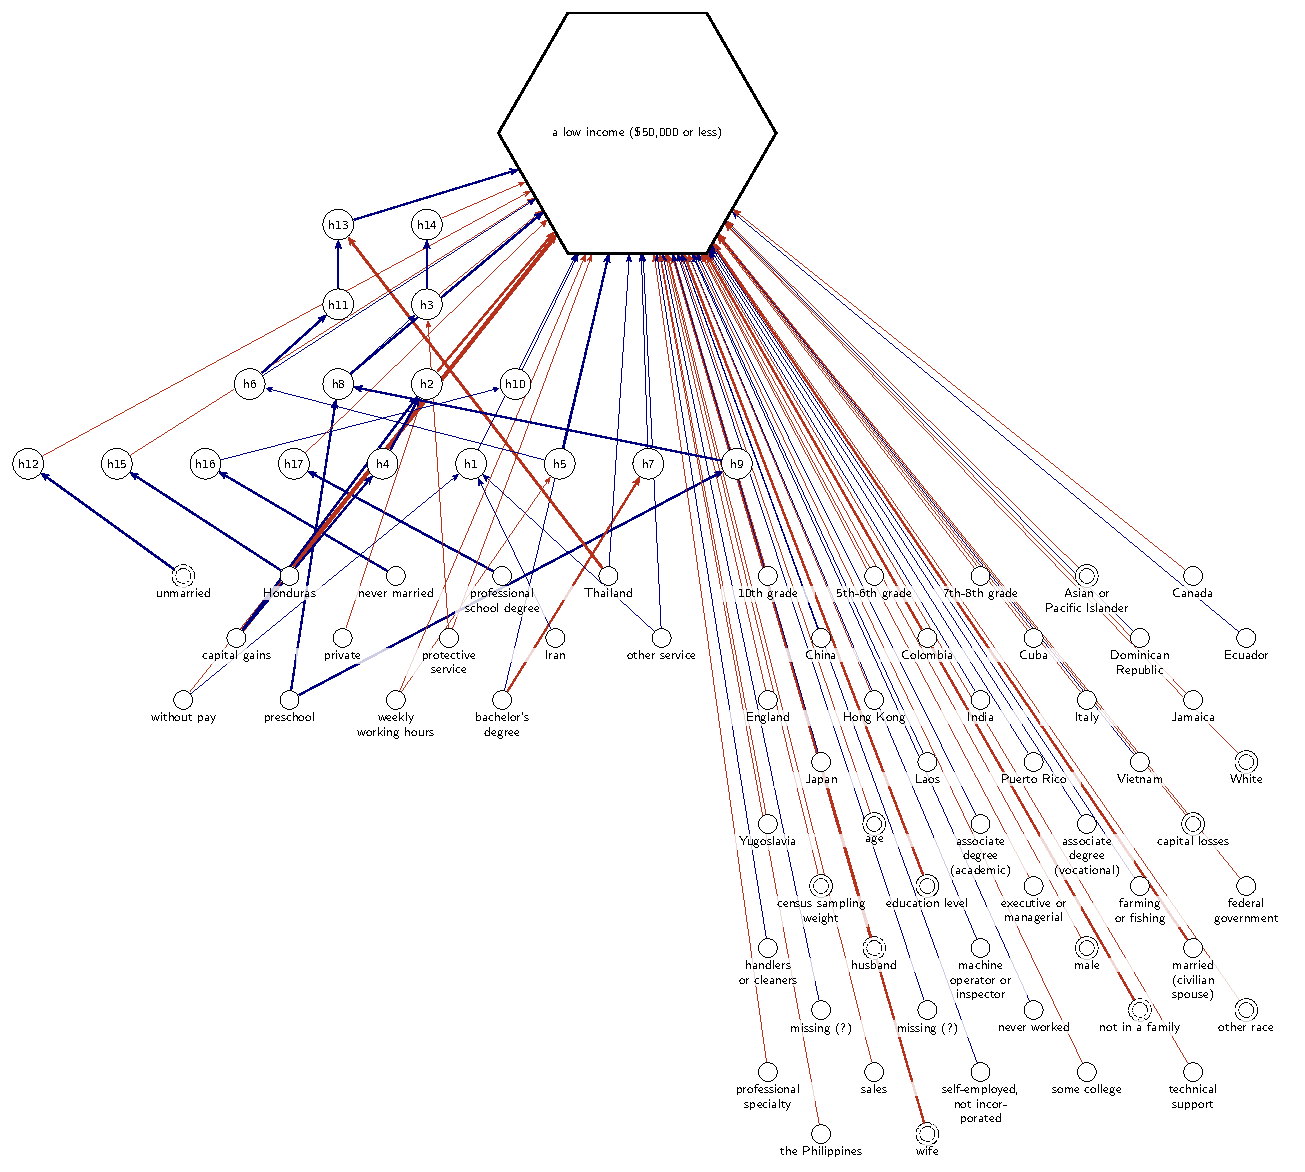
\includegraphics[width=\textheight,height=0.78\textwidth,keepaspectratio]{figures/exp2/networks/adult-s9-raw}
  \caption{Adult, seed 9 (adult-s9): the network as trained, before any explanation, in full. Inputs at the bottom (every input column its own node), hidden units by depth, the output at the top; 61 of 107 input columns are connected, with 17 hidden units and 91 enabled connections. Blue: positive weight (raises the score); red: negative weight (lowers it); thicker: larger weight. Orange outline and up arrow: raises the final prediction; teal and down arrow: lowers it; grey and double arrow: depends. Not used (no connection; 46 columns): local government, self-employed, incorporated, state government, 11th grade, doctorate, high-school graduate, master's degree, 12th grade (no diploma), 1st-4th grade, 9th grade, divorced, married to a member of the armed forces, married, spouse absent, separated, widowed, missing (?), administrative or clerical, transport or moving, armed forces, craft or repair, private household service, other relative, own child, American Indian or Eskimo, Black, Cambodia, France, Germany, Greece, Guatemala, Haiti, the Netherlands, Hungary, Ireland, Mexico, Nicaragua, outlying US territories (Guam, US Virgin Islands), Peru, Poland, Portugal, Scotland, 'South' (as recorded), Taiwan, Trinidad and Tobago, the United States and El Salvador.}
  \label{fig:exp2-net-adult-s9-raw}
\end{sidewaysfigure}
